\documentclass[12pt,onecolumn]{IEEEtran}

\usepackage[utf8]{inputenc}
\usepackage[T1]{fontenc}
\usepackage{graphicx}
\usepackage{booktabs}
\usepackage{tabularx}
\usepackage{array}
\usepackage{longtable}
\usepackage{multirow}
\usepackage{amsmath}
\usepackage{xcolor}
\usepackage{url}
\usepackage{hyperref}
\usepackage{enumitem}
\usepackage{float}
\usepackage{tikz}
\usetikzlibrary{arrows.meta,positioning,shapes.geometric,fit}

\hypersetup{
  colorlinks=true,
  linkcolor=blue!55!black,
  citecolor=blue!55!black,
  urlcolor=blue!55!black,
  pdftitle={First Signs: A Multilingual Multi-Syndrome Screening and Closed-Loop Care-Navigation Platform for Bangladesh},
  pdfauthor={Tawhidul Hasan}
}

\definecolor{fsblue}{HTML}{DDEEFF}
\definecolor{fsdark}{HTML}{172033}
\definecolor{fsgreen}{HTML}{DDF3E8}
\definecolor{fsamber}{HTML}{FBE8B5}
\definecolor{fsred}{HTML}{F8D7DA}
\newcommand{\product}{\textit{First Signs}}
\newcommand{\code}[1]{\texttt{#1}}
\newcommand{\repositorypath}[1]{\path{#1}}
\renewcommand{\arraystretch}{1.15}

\title{First Signs: A Multilingual Multi-Syndrome Screening and Closed-Loop Care-Navigation Platform for Bangladesh}

\author{Tawhidul Hasan%
\thanks{First Signs is a research and hackathon prototype. It is not a diagnostic system and has not received clinical or regulatory approval for public deployment.}%
}

\begin{document}
\maketitle

\begin{abstract}
This report presents the requirements, architecture, implementation, feasibility, and repository-level evaluation of \product, a multilingual, mobile-first screening and care-navigation prototype for Bangladesh. The system supports five non-diagnostic pathways: persistent cough or respiratory concern, fever or mosquito-borne illness concern, diarrhoea or dehydration concern, skin/sensation/nerve concern, and child cough or difficult breathing. Its central contribution is a closed-loop workflow that connects consent, deterministic warning-sign screening, facility discovery, optional referral, independent attendance verification, missed-visit follow-up, pharmacy-scoped simulated incentives, and privacy-preserving public-health signals. Safety outcomes are generated by fixed, versioned TypeScript rules; optional artificial intelligence and acoustic services are deliberately prevented from overriding them. The implementation uses Next.js 16, React 19, TypeScript, Supabase/PostgreSQL, MapLibre, QR tooling, optional Gemini assistance, Telegram messaging, Resend reminders, and a separately deployed Google HeAR service. Repository evaluation performed on 19 October 2026 found that ESLint, TypeScript checking, and the production build completed successfully and that 38 focused automated test cases passed. These results establish software consistency within the evaluated scope, not clinical effectiveness. The report concludes that the prototype is technically feasible for continued research, while real deployment remains contingent on clinical and Bangla-language review, verified multi-pathway facility data, accessibility and usability studies, operational partnerships, privacy governance, security testing, and prospective field evaluation.
\end{abstract}

\begin{IEEEkeywords}
digital health, care navigation, deterministic triage, multilingual health systems, Bangladesh, referral workflow, privacy, pharmacy engagement, public health, software engineering
\end{IEEEkeywords}

\section{Introduction}
People can be lost at several handoffs between noticing a warning sign and reaching formal care: interpreting symptoms, finding an appropriate service, preserving a referral, attending the visit, and recovering after a missed visit. Bangladesh research has documented delayed care seeking and frequent initial contact with nearby pharmacies among people with tuberculosis symptoms \cite{ahmed2025delay}. Related work also shows both the potential and the inconsistency of digital symptom checkers \cite{semigran2015symptom,wallace2022accuracy,riboli2023triage}. These findings motivate a system that is explicit about its limits and optimized for navigation rather than diagnosis.

\product addresses this gap with a single accountable journey:
\begin{center}
\textbf{Concern $\rightarrow$ safe guidance $\rightarrow$ facility $\rightarrow$ referral $\rightarrow$ attendance $\rightarrow$ follow-up.}
\end{center}
The system is multilingual in architecture and currently implements English and Bangla. It treats all five care pathways as first-class entry points. Disease-specific components---such as respiratory audio research and the current TB-evaluation facility directory---remain bounded to their relevant pathway and do not define the identity of the platform.

The report makes four contributions. First, it translates the product requirements and implementation into a structured software-engineering specification. Second, it documents the safety, privacy, incentive, and failure boundaries. Third, it places the work against peer-reviewed studies and digital-health guidance. Fourth, it reports reproducible repository-level verification without overstating those checks as clinical evidence.

\section{Background and Related Work}
\subsection{Digital triage and the case for deterministic navigation}
The research title \emph{Evaluation of Symptom Checkers for Self Diagnosis and Triage: Audit Study} reported substantial variation in diagnostic and triage performance across publicly available systems \cite{semigran2015symptom}. Later reviews---\emph{The Diagnostic and Triage Accuracy of Digital and Online Symptom Checker Tools: A Systematic Review} \cite{wallace2022accuracy} and \emph{Triage and Diagnostic Accuracy of Online Symptom Checkers: Systematic Review} \cite{riboli2023triage}---also found variable performance and limited evidence for safe broad adoption. This evidence supports the design choice in \product: a small, reviewable, versioned rules layer produces care-action categories, while generative AI is limited to bounded explanation and navigation.

The World Health Organization (WHO) similarly emphasizes that digital interventions supplement rather than replace health systems \cite{who2019digital}. WHO SMART Guidelines promote standards-based, machine-readable, adaptive, requirements-based, and testable specifications \cite{whoSmart}. \product follows this direction conceptually through language-neutral outcome codes, versioned rules, shared server validation, and testable care-pathway definitions, although it is not presented as a formal WHO SMART Guidelines implementation.

\subsection{Care seeking, pharmacies, and navigation}
The Bangladesh paper \emph{Mixed-methods Study to Assess Delay among Patients with Tuberculosis in an Urban Setting of Bangladesh} found delayed care seeking and identified nearby pharmacies as a frequent initial care contact \cite{ahmed2025delay}. In India, \emph{Can Community Pharmacists Improve Tuberculosis Case Finding? A Mixed Methods Intervention Study in India} evaluated pharmacy training, referrals, incentives, reminders, and field support \cite{daftary2019pharmacy}. The title \emph{Can Patient Navigators Help Potential TB Patients Navigate the Diagnostic and Treatment Pathways? An Implementation Research from India} further highlights the value of navigation across fragmented care journeys \cite{nayyar2021navigators}.

\product extends the workflow idea beyond a single condition while separating responsibilities: pharmacies may assist access, facilities independently confirm attendance, and rewards are limited to pharmacy-assisted workflow milestones. The prototype does not reward disease positivity and does not allow a pharmacy to verify its own referral.

\subsection{Research across the five pathways}
Table~\ref{tab:related} lists research-paper titles directly relevant to the design space. The comparison is thematic; it does not claim equivalence of populations, outcomes, or validation quality.

\begin{longtable}{p{0.24\textwidth}p{0.48\textwidth}p{0.22\textwidth}}
\caption{Related research papers and their relevance to \product.}\label{tab:related}\\
\toprule
Area & Research-paper title & Relevance to this work \\
\midrule
\endfirsthead
\toprule
Area & Research-paper title & Relevance to this work \\
\midrule
\endhead
Respiratory/TB & \emph{Mixed-methods Study to Assess Delay among Patients with Tuberculosis in an Urban Setting of Bangladesh} \cite{ahmed2025delay} & Care delays, pharmacy contact, and Bangladesh context. \\
Pharmacy referral & \emph{Can Community Pharmacists Improve Tuberculosis Case Finding? A Mixed Methods Intervention Study in India} \cite{daftary2019pharmacy} & Assisted screening, referral completion, and incentive feasibility. \\
Fever/dengue & \emph{District-Level Dengue Early Warning Prediction System in Bangladesh Using Hybrid Explainable AI and Bayesian Deep Learning} \cite{shiddik2026dengue} & Demonstrates district-level surveillance research; unlike \product, it uses confirmed historical case data and predictive modelling. \\
Fever/malaria & \emph{Knowledge on the Transmission, Prevention and Treatment of Malaria among Two Endemic Populations of Bangladesh and Their Health-Seeking Behaviour} \cite{haque2009malaria} & Shows knowledge, self-treatment, drug-seller contact, and delayed care-seeking challenges. \\
Diarrhoea & \emph{Effects of a Water, Sanitation, and Hygiene Mobile Health Program on Diarrhea and Child Growth in Bangladesh: A Cluster-Randomized Controlled Trial of the CHoBI7 Mobile Health Program} \cite{george2021chobi7} & Bangladesh evidence for mobile follow-up and behaviour-support messaging. \\
Skin/leprosy & \emph{Leprosy Screening Based on Artificial Intelligence: Development of a Cross-Platform App} \cite{desouza2021leprosy} & Illustrates mobile screening research and the need for population-specific validation; \product intentionally avoids visual diagnosis. \\
Bangladesh feasibility & \emph{Efficacy of Using a Digital Health Intervention Model Using Community Health Workers for Primary Health Services in Bangladesh: A Repeated Cross-Sectional Observational Study} \cite{zaman2025bangladesh} & Supports investigation of assisted digital-health delivery while not validating this prototype. \\
Health acoustics & \emph{HeAR---Health Acoustic Representations} \cite{baur2024hear} & Motivates optional acoustic embeddings; it does not justify a patient-level diagnosis or local clinical deployment. \\
Digital triage & \emph{Triage and Diagnostic Accuracy of Online Symptom Checkers: Systematic Review} \cite{riboli2023triage} & Supports conservative, non-diagnostic, auditable care navigation. \\
\bottomrule
\end{longtable}

\subsection{Comparative positioning}
The distinguishing unit in \product is the closed loop, not a new diagnostic model. Table~\ref{tab:comparison} compares architectural archetypes rather than claiming a controlled head-to-head product evaluation.

\begin{table}[H]
\caption{Conceptual comparison with common digital-health archetypes.}
\label{tab:comparison}
\centering
\small
\begin{tabularx}{\textwidth}{>{\raggedright\arraybackslash}p{0.19\textwidth}*{5}{>{\centering\arraybackslash}X}}
\toprule
Capability & Symptom checker & Health chatbot & Referral registry & Surveillance dashboard & \product \\
\midrule
Non-diagnostic warning-sign guidance & Sometimes & Sometimes & No & No & Yes \\
Deterministic urgent precedence & Variable & Variable & No & No & Yes \\
Multi-pathway patient flow & Usually & Usually & Limited & Aggregate only & Five pathways \\
Portable referral and QR & Rare & Rare & Yes & No & Yes \\
Independent attendance confirmation & Rare & Rare & Yes & No & Yes \\
Missed-visit barrier recovery & Limited & Limited & Sometimes & No & Yes \\
Pharmacy/self-use separation & Rare & Rare & Sometimes & No & Yes \\
Privacy-safe grouped signals & Rare & Rare & Sometimes & Yes & Yes \\
Optional services fail without changing safety outcome & Variable & Variable & N/A & N/A & Required \\
\bottomrule
\end{tabularx}
\end{table}

\section{Problem Definition and Objectives}
The primary problem is discontinuity between early concern and completed formal evaluation. The system objective is therefore not to infer disease probability, but to reduce avoidable loss at each transition. Secondary objectives are to support assisted access, retain patient control over referral creation, provide barrier-specific follow-up, make workflow participation auditable, and expose only minimum grouped signals for public-health investigation.

The design is constrained by six non-negotiable properties:
\begin{enumerate}[leftmargin=*]
  \item screening and navigation must never be presented as diagnosis;
  \item urgent danger signs take precedence over other results;
  \item incomplete or malformed answers do not yield a reassuring outcome;
  \item AI and acoustic services cannot create, downgrade, or reverse fixed safety outcomes;
  \item self-use and pharmacy-assisted incentive flows remain separate; and
  \item public-health views exclude identity, raw answers, referral tokens, audio, and exact GPS.
\end{enumerate}

\section{Requirement Analysis}
\subsection{Stakeholders and use cases}
The principal stakeholders are the person seeking care, assisting pharmacy staff, assigned facility staff, public-health viewers, platform administrators, and clinical/public-health reviewers. Optional AI, messaging, email, mapping, and audio providers are supporting services, not safety authorities.

\begin{table}[H]
\caption{Stakeholder requirements and access boundaries.}
\label{tab:stakeholders}
\centering
\small
\begin{tabularx}{\textwidth}{p{0.18\textwidth}X X}
\toprule
Stakeholder & Required capability & Explicit boundary \\
\midrule
Person & Consent, select pathway, answer questions, receive guidance, choose facility/referral, review own journey & Cannot view another person's care record; retains referral choice \\
Pharmacy & Assist a linked journey; view its own aggregate workflow and simulated credits & Cannot see self-use records, diagnose, or confirm attendance \\
Facility staff & Lookup an intended referral and confirm attendance once & Cannot control pharmacy rewards or record an app-generated diagnosis \\
Public health & View grouped programme indicators and broad-area signals & No patient identity, raw answers, exact GPS, token, or audio \\
Administrator & Invite and scope staff; review aggregate operations & No authority to change fixed clinical rules through AI \\
Optional services & Explain, route, message, email, map, or process transient audio & Failure must not change the deterministic safety result \\
\bottomrule
\end{tabularx}
\end{table}

\subsection{Functional requirements}
The implemented functional scope includes: two entry modes; persistent English/Bangla switching; explicit consent; five pathway-specific rule sets; three language-neutral outcome levels; broad-area facility discovery; optional transient GPS routing; optional referral creation; public referral ID plus private token; QR display and local scanning; independent one-time attendance verification; private My Care state; missed-visit barrier capture; pharmacy aggregates and simulated credits; duplicate/reuse/volume safeguards; grouped public-health signals; anonymous community feedback; optional accounts; a bounded health assistant; Medicine Corner; reminders; Telegram; and optional respiratory audio processing.

\subsection{Non-functional requirements}
Non-functional requirements include mobile-first responsiveness, accessibility, plain language, consistent English and Bangla meaning, prescribed typography, server-side validation, least-data collection, role and scope enforcement, transactional/idempotent writes, graceful degradation of optional services, secret isolation, low-coupling shared logic, and regression-testability. The project requires Merriweather for English and Noto Sans Bengali for Bangla. Important health information must not use light weights.

\subsection{Traceability}
\begin{table}[H]
\caption{Representative requirement-to-evidence traceability.}
\label{tab:traceability}
\centering
\small
\begin{tabularx}{\textwidth}{p{0.27\textwidth}p{0.36\textwidth}X}
\toprule
Requirement & Implementation evidence & Verification evidence \\
\midrule
Five deterministic pathways & \repositorypath{lib/care-pathways.ts} & \repositorypath{scripts/check-care-pathways.test.mts} \\
Respiratory urgent precedence & \repositorypath{lib/safety-rules.ts} & \repositorypath{scripts/check-safety-rules.test.mts} \\
Server screening validation & \repositorypath{app/api/screenings/route.ts} & Pathway and integration checks \\
Transactional referral numbering & Migration \repositorypath{20260912192242_use_transactional_referral_counter.sql} & \repositorypath{supabase/tests/referral_counter_invariants.sql} \\
Independent verification & \repositorypath{app/api/referrals/verify/route.ts} & \repositorypath{scripts/check-verification-flow.mjs} \\
Grouped public-health data & \repositorypath{app/api/dashboard/route.ts} and \repositorypath{lib/government-dashboard.ts} & Dashboard and SQL privacy checks \\
AI claim guardrails & \repositorypath{lib/ai-companion.ts} & \repositorypath{scripts/check-ai-companion.test.mts} \\
Transient audio hashing & \repositorypath{lib/audio-hash.ts} & \repositorypath{scripts/check-part14-audio-hash.test.mts} \\
\bottomrule
\end{tabularx}
\end{table}

\section{Methodology}
The development method is requirements-driven and safety-first. Product requirements in \repositorypath{PRD.md} take precedence over implementation guidance. The process used for the current codebase can be summarized as follows:
\begin{enumerate}[leftmargin=*]
  \item identify pathway-specific danger signs and care-navigation outputs;
  \item encode outcomes as language-neutral, deterministic rules with urgent precedence;
  \item keep translated presentation separate from the rule result;
  \item validate complete inputs on both client and server boundaries;
  \item persist private care records separately from minimum anonymous signals;
  \item implement referrals, verification, follow-up, and rewards as controlled state transitions;
  \item isolate optional AI, audio, messaging, mapping, and email integrations;
  \item add unit, API, browser, and database regression checks; and
  \item document limitations, mocked states, and deployment prerequisites.
\end{enumerate}

This method intentionally rejects an end-to-end opaque predictor. The design treats explainability as inspectability: a reviewer can locate the rule version, inputs, precedence, outcome code, display copy, API validation, migration, and regression test.

\section{Design Approach}
\subsection{Layered safety architecture}
The architecture separates the mandatory care path from optional enhancements. Figure~\ref{fig:architecture} shows the principal components and trust boundaries.

\begin{figure}[H]
\centering
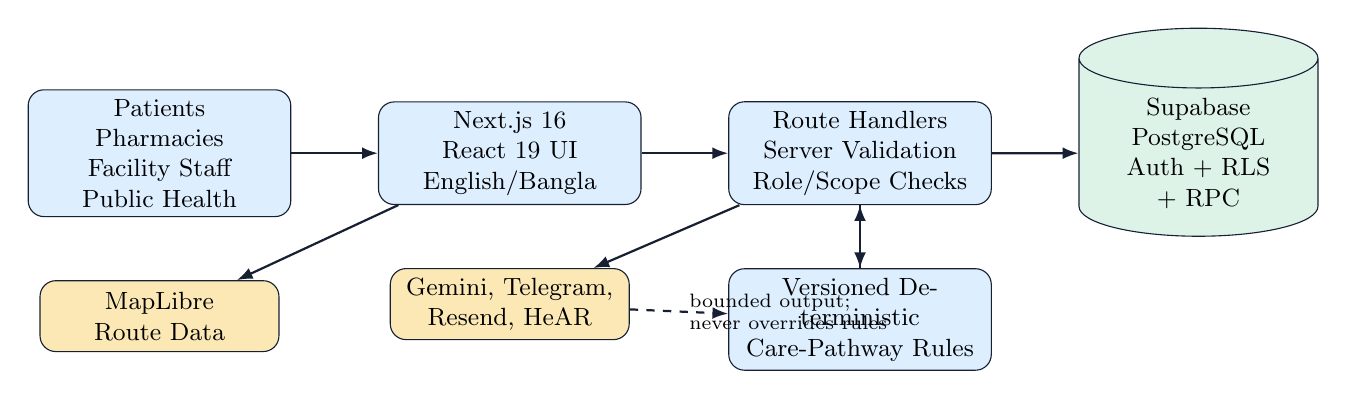
\begin{tikzpicture}[
  node distance=8mm and 11mm,
  box/.style={draw=fsdark, rounded corners=2mm, fill=fsblue, align=center, minimum height=9mm, text width=31mm, font=\small},
  data/.style={draw=fsdark, cylinder, shape border rotate=90, aspect=0.25, fill=fsgreen, align=center, minimum height=13mm, text width=28mm, font=\small},
  ext/.style={draw=fsdark, rounded corners=2mm, fill=fsamber, align=center, minimum height=9mm, text width=28mm, font=\small},
  arrow/.style={-{Latex[length=2mm]}, thick, draw=fsdark}
]
\node[box] (users) {Patients\\Pharmacies\\Facility Staff\\Public Health};
\node[box, right=of users] (ui) {Next.js 16\\React 19 UI\\English/Bangla};
\node[box, right=of ui] (api) {Route Handlers\\Server Validation\\Role/Scope Checks};
\node[box, below=of api] (rules) {Versioned Deterministic\\Care-Pathway Rules};
\node[data, right=of api] (db) {Supabase\\PostgreSQL\\Auth + RLS + RPC};
\node[ext, below=of users] (maps) {MapLibre\\Route Data};
\node[ext, below=of ui] (optional) {Gemini, Telegram,\\Resend, HeAR};
\draw[arrow] (users) -- (ui);
\draw[arrow] (ui) -- (api);
\draw[arrow] (api) -- (db);
\draw[arrow] (api) -- (rules);
\draw[arrow] (rules) -- (api);
\draw[arrow] (ui) -- (maps);
\draw[arrow] (api) -- (optional);
\draw[arrow, dashed] (optional) -- node[right, font=\scriptsize, align=left]{bounded output;\\never overrides rules} (rules);
\end{tikzpicture}
\caption{System architecture and safety boundary. Optional services may support access or explanation, but deterministic rules remain authoritative for care guidance.}
\label{fig:architecture}
\end{figure}

\subsection{End-to-end workflow}
\begin{figure}[H]
\centering
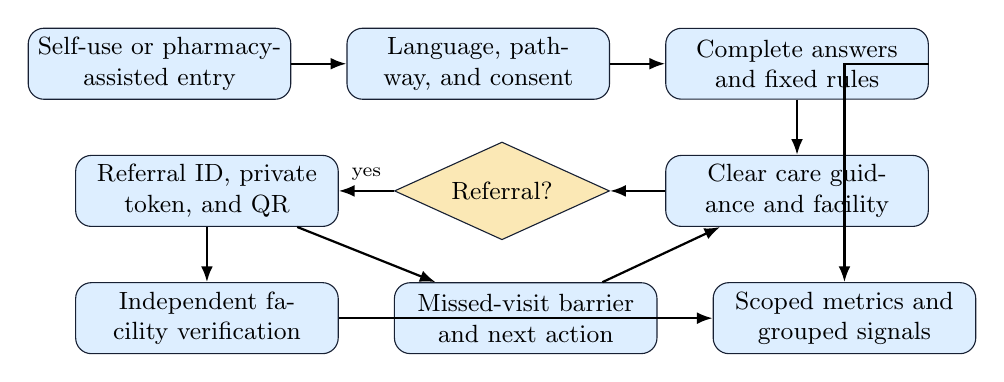
\begin{tikzpicture}[
  node distance=7mm,
  stage/.style={draw=fsdark, rounded corners=2mm, fill=fsblue, align=center, minimum height=9mm, text width=31mm, font=\small},
  decision/.style={draw=fsdark, diamond, aspect=2.2, fill=fsamber, align=center, inner sep=1.5mm, font=\small},
  arrow/.style={-{Latex[length=2mm]}, thick}
]
\node[stage] (entry) {Self-use or pharmacy-assisted entry};
\node[stage, right=of entry] (consent) {Language, pathway, and consent};
\node[stage, right=of consent] (screen) {Complete answers and fixed rules};
\node[stage, below=of screen] (guidance) {Clear care guidance and facility};
\node[decision, left=of guidance] (refer) {Referral?};
\node[stage, left=of refer] (ticket) {Referral ID, private token, and QR};
\node[stage, below=of ticket] (verify) {Independent facility verification};
\node[stage, right=of verify] (followup) {Missed-visit barrier and next action};
\node[stage, right=of followup] (aggregate) {Scoped metrics and grouped signals};
\draw[arrow] (entry) -- (consent);
\draw[arrow] (consent) -- (screen);
\draw[arrow] (screen) -- (guidance);
\draw[arrow] (guidance) -- (refer);
\draw[arrow] (refer) -- node[above, font=\scriptsize]{yes} (ticket);
\draw[arrow] (ticket) -- (verify);
\draw[arrow] (ticket) -- (followup);
\draw[arrow] (followup) -- (guidance);
\draw[arrow] (verify) -- (aggregate);
\draw[arrow] (screen.east) -| (aggregate.north);
\end{tikzpicture}
\caption{Closed-loop care journey. Referral remains a patient choice; urgent instructions remain visible even when referral is declined.}
\label{fig:workflow}
\end{figure}

\subsection{Data and privacy design}
Private care state and public-health signals are deliberately separated. Private records may include consented answers, care outcome, referral state, intended facility, and follow-up status. The signal path retains only approved minimum dimensions such as pathway, age band, broad area, entry type, outcome, and time. Exact GPS may be used transiently for route drawing but is not persisted in screening, referral, analytics, or hotspot records. Raw audio and embeddings are transient in the documented workflow. Telegram continuity uses a one-way channel identifier. Reminder email content is generic.

Supabase Auth provides account sessions; server routes resolve effective role and scope. PostgreSQL functions support controlled state changes and idempotency. Row-level security is enabled on exposed tables, while privileged server credentials remain outside the browser. The codebase uses a browser-safe publishable key only for client authentication and keeps the secret/service-role key server-side.

\subsection{Interface design}
The interface is mobile-first and uses a restrained claymorphic language: pale-blue shells, white navigation, black pill actions, soft-gray cards, clear status surfaces, generous spacing, and limited motion. English uses Merriweather and Bangla uses Noto Sans Bengali. The UI emphasizes readable health actions rather than decorative depth.

\begin{figure}[H]
\centering
\begin{minipage}{0.48\textwidth}
  \centering
  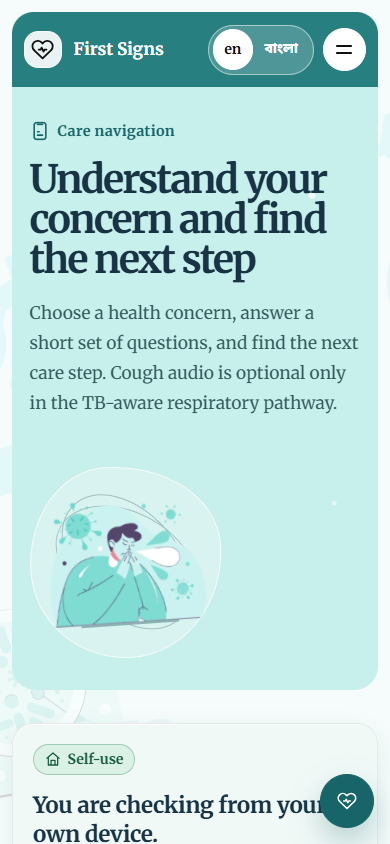
\includegraphics[width=0.92\linewidth]{../images/first-signs-screening.png}
  \small English screening entry
\end{minipage}\hfill
\begin{minipage}{0.48\textwidth}
  \centering
  
\includegraphics[width=0.92\linewidth]{../images/first-signs-screening-bangla.png}
  \small Bangla screening entry
\end{minipage}
\caption{The current multilingual implementation supports English and Bangla through the same shared workflow.}
\label{fig:languages}
\end{figure}

\section{Implementation and Software Engineering Work}
\subsection{Technology stack}
\begin{table}[H]
\caption{Implemented technology stack and responsibility.}
\label{tab:stack}
\centering
\small
\begin{tabularx}{\textwidth}{p{0.19\textwidth}p{0.25\textwidth}X}
\toprule
Layer & Technology & Responsibility \\
\midrule
Web & Next.js 16.3.8, React 19.2.8 & App Router pages, server rendering, route handlers, interactive workflows \\
Language & TypeScript 5.9 strict mode & Shared types, validation, deterministic care rules \\
Data/auth & Supabase, PostgreSQL, \code{@supabase/ssr} & Auth, persistence, RLS, transactional functions, scoped aggregates \\
Mapping & MapLibre GL JS 6.9 & Facility maps, routes, broad-area visualization \\
Motion & Motion 14.3 & Restrained transitions with reduced-motion support \\
Referral & \code{qrcode}, \code{jsqr} & QR generation and local image parsing \\
AI & Gemini API, bounded retrieval layer & Optional approved-source explanations; no safety authority \\
Messaging & Telegram Bot API & Optional alternate entry channel and status/follow-up commands \\
Email & Resend & Optional generic reminders \\
Audio & Separate Python/HeAR service & Optional transient cough-like-signal processing \\
Testing & Node test runner, Playwright Core & Unit, integration, browser, language, and responsive checks \\
\bottomrule
\end{tabularx}
\end{table}

\subsection{Repository structure and scale}
At the time of analysis, the scoped application, component, library, script, database, audio-service, and documentation directories contained 56 TypeScript files, 38 TSX files, 43 SQL files, 21 MJS files, 8 MTS files, and 9 Python files. The source tree includes 13 user-facing page modules, 21 API/callback route modules, 33 ordered Supabase migrations, and 36 test/check artifacts. These counts describe repository structure, not code quality by themselves.

Core modules include \repositorypath{lib/care-pathways.ts}, \repositorypath{components/screening-flow.tsx}, \repositorypath{lib/care-session.ts}, \repositorypath{lib/auth.ts}, \repositorypath{lib/supabase-server.ts}, \repositorypath{lib/health-rag.ts}, and \repositorypath{lib/messaging-server.ts}. The API surface covers screenings, signals, referrals, verification, follow-up, care state, accounts, authentication, reminders, dashboards, community feedback, medicines, health assistance, audio, invitations, and Telegram webhooks.

\subsection{Deterministic care rules}
Each pathway returns one of three language-neutral outcomes:
\begin{align*}
O \in \{&\texttt{CONTINUE\_WITH\_CARE\_INFORMATION},\\
        &\texttt{PROFESSIONAL\_EVALUATION\_RECOMMENDED},\\
        &\texttt{URGENT\_MEDICAL\_EVALUATION}\}.
\end{align*}
For every pathway, any true urgent question is checked before non-urgent referral criteria. The respiratory path additionally validates cough duration and checks the documented 14-day boundary. The fever path does not infer dengue instead of malaria. The skin/nerve path does not diagnose leprosy. The child-breathing path does not label pneumonia, and adults selecting it receive general evaluation guidance.

\subsection{Transaction and integrity design}
Referral creation uses a public-facing identifier and opaque private token. A database counter ensures that rolled-back requests and idempotent retries do not consume identifiers. Attendance completion is one-time and idempotent. Pharmacy rewards are evaluated independently of safety outcomes and only for validated pharmacy-assisted cases. Duplicate patient reward windows, repeated audio hashes, referral reuse, and unusual activity produce narrow blocks or review states rather than blocking care.

\subsection{Failure engineering}
The project uses explicit safe degradation. If Gemini is unavailable, fixed screening and referral still work. If HeAR decoding, inference, or connectivity fails, the symptom-based path continues. If route drawing fails, facility details remain available. If reminder delivery fails, referral state does not change. Server requests reject malformed or incomplete answers instead of silently coercing them.

\section{Feasibility Study}
\subsection{Technical feasibility}
Technical feasibility is supported by a successful production build, typed shared logic, route-level validation, ordered migrations, and focused automated checks. The stack is conventional for a web prototype and can run on Node-compatible hosting with a managed PostgreSQL service. Optional services are isolated and therefore do not form a single point of failure for safety guidance.

\subsection{Operational feasibility}
The two entry modes address both independent smartphone use and assisted access. QR referrals reduce reliance on verbal handoffs; My Care and follow-up preserve continuity after a missed visit. However, operational feasibility depends on verified facilities, staff onboarding, reliable identity and authorization, referral acceptance, support ownership, and service-level agreements. The current temporary staff PIN and laptop/tunnel audio deployment are demonstration mechanisms, not production operations.

\subsection{Clinical feasibility}
The rule architecture is reviewable, but clinical feasibility is not yet established. Every question, danger sign, threshold, translation, facility mapping, and care message requires qualified review. Prospective studies must measure under-triage, over-triage, comprehension, adherence, and unintended effects. No repository test establishes sensitivity, specificity, clinical benefit, or safety in a patient population.

\subsection{Economic feasibility}
The core software uses widely available open-source components and managed-service tiers, which is favourable for prototyping. Costs remain uncertain for production database capacity, SMS/email/messaging, maps/routes, support staff, facility verification, security monitoring, incident response, clinical governance, and incentive funding. The pharmacy credits are illustrative; no cost-effectiveness or real-payment model has been evaluated.

\subsection{Privacy, legal, and governance feasibility}
Data minimization, broad-area signals, RLS, server-only secrets, and role-scoped APIs provide a useful foundation. Deployment would still require a formal data-protection impact assessment, threat modelling, retention schedules, consent governance, breach response, vendor agreements, regulatory classification, and review under applicable Bangladesh law and health-sector policy.

\begin{table}[H]
\caption{Feasibility summary.}
\label{tab:feasibility}
\centering
\small
\begin{tabularx}{\textwidth}{p{0.17\textwidth}p{0.19\textwidth}X}
\toprule
Dimension & Current assessment & Evidence and next gate \\
\midrule
Technical & Feasible prototype & Build and focused tests pass; validate live DB/browser/external-service flows \\
Operational & Partially feasible & Complete workflow exists; requires partners, verified facilities, production staff identity, and support ownership \\
Clinical & Not established & Deterministic design is auditable; requires expert review and prospective validation \\
Economic & Unknown & Open-source base; no deployment costing, incentive financing, or cost-effectiveness study \\
Privacy/governance & Promising design, incomplete assurance & Data-minimization controls exist; requires formal legal, security, retention, and incident governance \\
Scale & Plausible, untested & Managed web/database architecture; no load, availability, or nationwide field study \\
\bottomrule
\end{tabularx}
\end{table}

\section{Results and Experiments}
\subsection{Evaluation protocol}
Repository checks were executed on 19 October 2026 in the project workspace. Commands were invoked with Windows command shims because local PowerShell policy blocked the \code{npm.ps1} and \code{npx.ps1} wrappers before project execution. The evaluated commands were:
\begin{itemize}[leftmargin=*]
  \item \code{npm.cmd run lint};
  \item \code{npx.cmd tsc --noEmit};
  \item \code{npm.cmd run build}; and
  \item focused suites for pathway rules, respiratory safety, configuration, audio hashing, AI guardrails, medicine data, and messaging security.
\end{itemize}

\subsection{Observed results}
ESLint completed with no reported errors, TypeScript checking completed successfully, and the Next.js 16.3.8 production build compiled, type-checked, generated static output, and listed the expected static and dynamic routes. Seven focused suites executed 38 test cases; all 38 passed, with no failed, cancelled, skipped, or todo cases.

\begin{table}[H]
\caption{Focused automated test results observed during report preparation.}
\label{tab:tests}
\centering
\small
\begin{tabularx}{\textwidth}{X r r r}
\toprule
Suite & Passed & Failed & Scope \\
\midrule
Care pathways & 6 & 0 & All five normal/referral/urgent paths; adult child-path boundary \\
Respiratory safety & 9 & 0 & 14-day boundary, symptoms, urgent precedence, invalid inputs \\
Server configuration & 5 & 0 & Secret-safe reporting and optional integration states \\
Audio hash & 2 & 0 & Standard SHA-256 vectors \\
AI guardrails & 5 & 0 & Barrier normalization and diagnostic-claim rejection \\
Medicine Corner & 2 & 0 & At least 100 unique entries and two-language safety/source data \\
Messaging & 9 & 0 & Source preservation, media validation, retry/privacy/host controls \\
\midrule
Total & 38 & 0 & Focused repository tests \\
\bottomrule
\end{tabularx}
\end{table}

\begin{figure}[H]
\centering
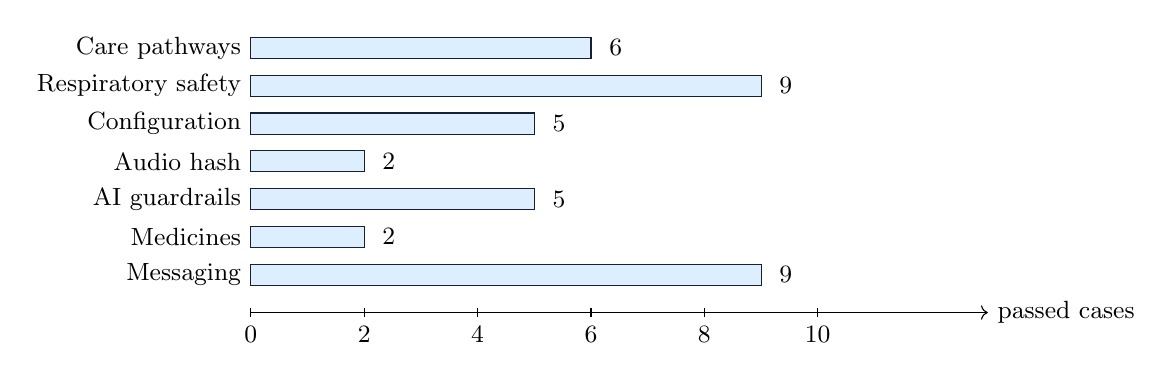
\begin{tikzpicture}[x=0.72cm,y=0.48cm,font=\small]
  \draw[->] (0,0) -- (13,0) node[right]{passed cases};
  \foreach \x in {0,2,4,6,8,10} {\draw (\x,0.12)--(\x,-0.12) node[below]{\x};}
  \foreach \y/\label/\value in {1/Messaging/9,2/Medicines/2,3/AI guardrails/5,4/Audio hash/2,5/Configuration/5,6/Respiratory safety/9,7/Care pathways/6} {
    \node[anchor=east] at (0,\y) {\label};
    \filldraw[fill=fsblue,draw=fsdark] (0,\y-0.28) rectangle (\value,\y+0.28);
    \node[anchor=west] at (\value+0.15,\y) {\value};
  }
\end{tikzpicture}
\caption{Focused test cases passed by suite. Counts are software tests, not patient or clinical observations.}
\label{fig:testbars}
\end{figure}

\subsection{Interpretation and threats to validity}
The results support internal consistency of the checked rules and utilities. They do not validate translations, care thresholds, clinical outcomes, live database policies, facility accuracy, third-party availability, accessibility, performance under load, or behaviour on the full range of low-cost devices. Browser suites, SQL regression tests, live Supabase integration, live Gemini/Telegram/Resend/HeAR checks, penetration testing, and human-subject studies were outside this report-preparation run. Some repository browser tests use controlled fixtures and should be interpreted as interface regression evidence, not external-service validation.

\section{Discussion}
\subsection{Why the closed loop matters}
Most digital-health components solve only one segment: information, triage, messaging, referral, or reporting. \product combines them while preserving role separation. A pathway result can lead to a destination; a referral can be independently completed; a missed visit can return to navigation; and programme signals can be derived without publishing private records. This creates a stronger basis for measuring referral acceptance and attendance than an isolated symptom questionnaire.

\subsection{Safety versus flexibility}
Deterministic rules trade predictive flexibility for auditability. For an early-stage, multi-pathway prototype, this is appropriate: urgent precedence, required-input checks, and language-neutral codes can be reviewed and regression-tested. AI remains useful for explanation and barrier normalization, but allowing it to set safety outcomes would expand the validation burden and introduce non-deterministic failure modes.

\subsection{Privacy versus public-health utility}
The design uses data minimization rather than attempting to anonymize a full patient record. Broad-area, pathway-level signals are useful for investigation and capacity planning but cannot establish disease prevalence or an outbreak. Synthetic thresholds shown in the prototype are demonstration rules only. A real programme would require statistical disclosure controls, minimum cell sizes, temporal smoothing, governance, and epidemiological validation.

\subsection{Equity and multilingual access}
English/Bangla switching, assisted entry, mobile-first layouts, and optional messaging address several access barriers. They do not eliminate inequity. Smartphone access, connectivity, literacy, disability, gendered phone access, staff behaviour, travel cost, and facility capacity can still determine whether guidance becomes care. Additional languages must be fully translated and clinically reviewed rather than added as partial interface overlays.

\section{Challenges}
The main engineering and research challenges are:
\begin{itemize}[leftmargin=*]
  \item preserving simple patient language without weakening urgent instructions;
  \item keeping five symptom-overlapping pathways distinct and non-diagnostic;
  \item guaranteeing equivalent meaning across languages and interface states;
  \item validating facility capability across Bangladesh, particularly outside the current TB-centred directory;
  \item protecting privacy while retaining useful programme signals;
  \item preventing incentives from distorting clinical behaviour;
  \item maintaining identical safety behaviour across web and messaging channels;
  \item operating optional external services without making them safety dependencies;
  \item governing audio data, dataset licences, calibration, and subgroup performance; and
  \item distinguishing a polished prototype from an approved clinical system.
\end{itemize}

\section{Limitations}
\product has not received clinical, public-health, accessibility, security, legal, or regulatory approval. English and Bangla content requires independent review. Facility availability may be outdated, and multi-pathway service coverage is incomplete. The staff PIN is prototype access separation rather than production identity management. Pharmacy rewards are simulated. Human-support escalation is a workflow marker and does not notify a real support team. The optional acoustic path is investigational and lacks the locally authorized clinical dataset, calibration, subgroup evaluation, and external validation required for patient-facing TB triage. Exact GPS is intentionally not persisted, which protects privacy but can limit continuity of route personalization. Grouped signals are not disease counts, prevalence estimates, or confirmed outbreaks. Finally, software test success cannot establish effectiveness, safety, adoption, or population benefit.

\section{Future Scope}
Prioritized future work includes:
\begin{enumerate}[leftmargin=*]
  \item independent clinical, public-health, and Bangla-language review of every pathway;
  \item usability and comprehension studies with patients, pharmacy workers, and facility staff;
  \item verified, regularly maintained, pathway-specific facility data across all divisions;
  \item stronger accessibility, offline/low-bandwidth behaviour, and low-cost-device testing;
  \item production-grade staff identity, organizational scoping, audit logs, and incident response;
  \item privacy thresholds and formal statistical-disclosure review for public-health reporting;
  \item prospective measurement of referral acceptance, attendance, time-to-care, barrier resolution, and inequities;
  \item controlled evaluation of pharmacy incentives under partner governance, including adverse incentives and cost-effectiveness;
  \item standards-based interoperability with health information exchanges and referral systems;
  \item additional fully reviewed languages with approved fonts and equivalent safety semantics;
  \item load, resilience, penetration, and disaster-recovery testing; and
  \item separately governed acoustic research using authorized data, preregistered evaluation, calibration, subgroup analysis, and external validation.
\end{enumerate}

\section{Conclusion}
\product demonstrates a technically coherent approach to multi-syndrome care navigation in Bangladesh. Its contribution is the integration of deterministic safety guidance with destination finding, optional portable referral, independent attendance confirmation, barrier-aware follow-up, scoped incentives, and privacy-safe programme signals. The repository exhibits meaningful software-engineering depth and passed the focused static, build, and unit checks executed for this report. The responsible conclusion is nevertheless limited: the codebase is a promising and testable prototype, not a diagnostic device or clinically validated service. The next stage should prioritize human review and field evidence over additional feature breadth.

\section*{Artifact Availability}
The source report is located at \repositorypath{docs/report/first-signs-ieee-report.tex}; references are in \repositorypath{docs/report/references.bib}. Repository-owned screenshots are loaded from \repositorypath{docs/images}. The report is configured with the IEEEtran class in explicit one-column mode.

\bibliographystyle{IEEEtran}
\bibliography{references}

\end{document}
